%!TEX root = main.tex

\section{The Frank-Wolfe Method}\index{Frank-Wolfe method}\index{Conditional-Gradient method|see {Frank-Wolfe method}}

Also known as the \emph{Conditional-Gradient method}, it is widely used to solve programs where the feasibility region $S$ is described by a system of linear inequalities.
\begin{equation*}
(P): \begin{cases} \displaystyle{\min_{\x\in S}f(\x)} \\ S=\{ \x \in \field{R}^d:  \langle \boldsymbol{a}_k, \x \rangle \leq b_k \text{ with } \boldsymbol{a}_k \in \field{R}^d, b_k \in \field{R}, 1\leq k \leq \ell  \}
\end{cases}
\end{equation*}

This is an iterative method that, at any feasible initial guess $\x_0 \in S$, considers an associated linear program $(LP_0)$ that minimizes the linear approximation $L_0(\x) = f(\x_0) + \langle \gradient{f}(\x_0), \x - \x_0 \rangle$ on the same feasible region $S$.
\begin{equation*}
(LP_0): \begin{cases} \displaystyle{\min_{\x \in S} \langle \gradient{f}(\x_0), \x-\x_0 \rangle} \\
 S =\{ \x \in \field{R}^d:  \langle \boldsymbol{a}_k, \x \rangle \leq b_k \text{ with } \boldsymbol{a}_k \in \field{R}^d, b_k \in \field{R}, 1\leq k \leq \ell  \}
 \end{cases}
\end{equation*}
Once an optimal solution $\bar{\x}_0$ of $(LP_0)$ has been obtained, a line-search\index{Line-search} is performed on the segment joining $\x_0$ with $\bar{\x}_0$ (which by hypothesis is contained in the feasibility region $S$). 
\begin{equation*}
t_0 = \argmin_{0\leq t \leq 1} f\big(\x_0 + t(\bar{\x}_0-\x_0) \big).
\end{equation*}
Set then $x_1 = \x_0 + t_0 (\bar{\x}_0-\x_0)$.  We repeat this process to obtain a sequence $\{\x_n\}_{n\in\field{N}}$ of feasible points.

We usually devise a \emph{stopping criteria} (given a fixed tolerance $\varepsilon>0$) to guarantee that we are close enough to the optimal solution of $(P)$.  An example of such a process is illustrated below:\index{Frank-Wolfe method!stopping criteria}\index{Frank-Wolfe method!lower bound}\index{Frank-Wolfe method!upper bound}
\begin{description}
\item [Initialization] Let $\x_0 \in S$ be an initial feasible guess, and set $LB=-\infty$, $UB=f(\x_0)$---the \emph{lower} and \emph{upper} bounds (respectively) for the stopping criteria.
\item [Iteration] Assume we have $\x_n$, $LB$, $UB$.  Set 
\begin{equation*}
L_n(\x) = f(\x_n) + \langle \gradient{f}(\x_n), \x-\x_n \rangle. 
\end{equation*}
Find
\begin{align*}
\bar{\x}_n &= \argmin_{\x \in S} L_n(\x) = \argmin_{\x \in S} \langle \gradient{f}(\x_n), \x-\x_n \rangle,\\
\xi_n &= \min_{\x \in S} L_n(\x) = L_n(\bar{\x}_n),\\
t_n &= \argmin_{0 \leq t \leq 1} f\big(\x_n + t(\bar{\x}_n - \x_n)\big), \\
\x_{n+1} &= \x_n + t_n (\bar{\x}_n - \x_n), \\
LB &= \max(LB, \xi_n)
\end{align*}
\item [Stopping Criteria] If $\lvert UB-LB \rvert \leq \varepsilon$, then stop. Otherwise, update the upper bound, $UB = f(\x_{n+1})$, and perform the next \textbf{Iteration}.
\end{description}

\begin{example}\label{example:FrankWolfe}
Let us use this technique to try and find the minimum value of the function $f(x,y)=(x-3)^2+(y-2)^2$ over the square with vertices at $(-3/2, 0)$, $(0, 3/2)$, $(3/2, 0)$ and $(0, -3/2)$. We start by defining the inequality constraints:
\begin{align*}
g_1(x,y) &= x+y-\tfrac{3}{2} = \langle [1,1], [x,y] \rangle - \tfrac{3}{2} \\
g_2(x,y) &= x-y-\tfrac{3}{2} = \langle [1,-1], [x,y] \rangle - \tfrac{3}{2} \\
g_3(x,y) &= -x-y-\tfrac{3}{2} = \langle [-1,-1], [x,y] \rangle - \tfrac{3}{2} \\
g_4(x,y) &= -x+y-\tfrac{3}{2} = \langle [-1,1], [x,y] \rangle - \tfrac{3}{2}
\end{align*}
\begin{figure}[ht!]
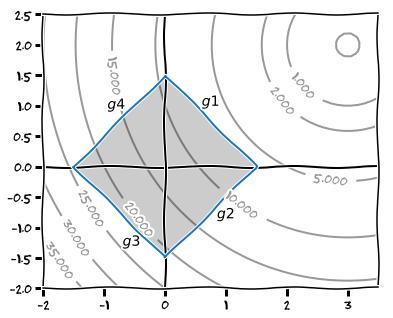
\includegraphics[width=0.75\linewidth]{images/frankwolfesetup.png}
\caption{Set up for Example \ref{example:FrankWolfe}}\label{figure:FrankWolfesetup}
\end{figure}
We also need the gradient of $f$: $\gradient{f}(x,y) = \big[ 2(x-3), 2(y-2) \big]$. At any point $(x_0,y_0)$, the linear approximation needed for this method is given by
\begin{align*}
L_0(x,y) &= f(x_0,y_0) + \langle \gradient{f}(x_0, y_0), (x-x_0,y-y_0) \rangle \\
&= (x_0-3)^2 + (y_0-2)^2 + 2(x_0-3)(x-x_0) + 2(y_0-2)(y-y_0).
\end{align*}
Let's assume that the initial guess is $(0,0)$, and we are looking for an exact solution ($\varepsilon=0$).  At this point, we set up $LB=-\infty$, and $UB=f(0,0)=13$.  According to our description of Frank-Wolfe, we have to solve at this step the program
\begin{equation*}
(LP_0): \begin{cases} \displaystyle{\min_{(x,y) \in S}} \big( -6x-4y \big) \\ S = \{ (x,y) \in \field{R}^2 : g_k(x,y) \leq 0, 1 \leq k \leq 4 \} \end{cases}
\end{equation*}
By performing the simplex method, we find the optimal solution of this program attained at the point $(\bar{x}_0, \bar{y}_0) = (3/2,0)$, with $\xi_0 = L_0(3/2,0) = -9$. We proceed to perform a line-search on the segment joining $(0,0)$ and $(3/2,0)$:
\begin{equation*}
t_0 = \argmin_{0 \leq t \leq 1} f\big(\tfrac{3}{2}t, 0 \big) = \argmin_{0 \leq t \leq 1} \big[ 4 + \big(\tfrac{3}{2}t-3 \big)^2 \big] = 1.
\end{equation*}
It is then $(x_1,y_1)=(x_0,y_0)+t_0(\bar{x}_0-x_0, \bar{y}_0 - y_0) = \big( \tfrac{3}{2}, 0 \big)$, and $LB=\max(-\infty, \xi_0)=-9$.

At this point the stopping criteria gives $\lvert UB - LB \rvert = \lvert 13-(-9) \rvert = 22$.  We proceed to the second iteration step, but we update the upper bound first: $UB=f(x_1,y_1)=f(3/2,0)=25/4$.

We need the approximation to $f$ at $(3/2,0)$: 
\begin{align*}
L_1(x,y) &= f\big( \tfrac{3}{2} ,0\big) + \big\langle \gradient{f}\big( \tfrac{3}{2},0 \big), \big[ x-\tfrac{3}{2}, y \big] \big\rangle \\
&= \tfrac{25}{4} + \big\langle [-3,-4], \big[ x-\tfrac{3}{2}, y \big] \big\rangle = \tfrac{25}{4} - 3\big( x-\tfrac{3}{2} \big) - 4y
\end{align*}
The corresponding associated program at this stage is as follows:
\begin{equation*}
(LP_1): \begin{cases} 
\displaystyle{\min_{(x,y) \in S}} \big( -3x-4y \big) \\
S = \{ (x,y) \in \field{R}^2 : g_k(x,y) \leq 0, 1 \leq k \leq 4 \}
\end{cases}
\end{equation*}
After applying the simplex method to this program, we find that the solution is the point $(\bar{x}_1, \bar{y}_1) = (0,3/2)$, with $\xi_1 = L_1(0,3/2) = 19/4$.

A line search between $(x_1,y_1)$ and $(\bar{x}_1, \bar{y}_1)$ gives
\begin{equation*}
t_1 = \argmin_{0 \leq t \leq 1} f\big( \tfrac{3}{2}(1-t), \tfrac{3}{2}t \big) = \argmin_{0 \leq t \leq 1} \big( \tfrac{9}{2}t^2 - \tfrac{3}{2}t + \tfrac{25}{4} \big) = \tfrac{1}{6},
\end{equation*}
and therefore $(x_2,y_2) = (x_1,y_1)+t(\bar{x}_1-x_1, \bar{y}_1-y_1) = (5/4, 1/4)$. We also have $LB = \max( -9, \xi_1 ) = 19/4$.  

At this point, the stopping criteria gives $\lvert UB - LB \rvert = \lvert 25/4 - 19/4 \rvert = \tfrac{3}{2}$.  We proceed to the third step, but update the upper bound first: $UB=f(x_2,y_2)=f(5/4,1/4)=49/8$.

We need the approximation to $f$ at $(5/4, 1/4)$:
\begin{equation*}
L_2(x,y) = f\big(\tfrac{5}{4}, \tfrac{1}{4} \big) + \big\langle \gradient{f}(\tfrac{5}{4}, \tfrac{1}{4} \big), \big[ x - \tfrac{5}{4}, y-\tfrac{1}{4} \big] \big\rangle = -\tfrac{7}{2}x -\tfrac{7}{2}y + \tfrac{91}{8}.
\end{equation*}
The corresponding associated program at this stage is as follows:
\begin{equation*}
(LP_2): \begin{cases}
\displaystyle{\min_{(x,y) \in S}} \big( -\tfrac{7}{2}x -\tfrac{7}{2}y \big) \\
S = \{ (x,y) \in \field{R}^2 : g_k(x,y) \leq 0, 1 \leq k \leq 4 \}
\end{cases}
\end{equation*}
The solution is again the point $(\bar{x}_2, \bar{y}_2) = (5/4, 1/4)$, with $\xi_2 = L_2(5/4,1/4) = 49/8$.  No further computations are needed at this point to realize that $(x_3,y_3)=(\bar{x}_2, \bar{y}_2)=(x_2,y_2)=(5/4, 1/4)$.  Notice that $\lvert UB-LB \rvert=0$, and the stopping criteria has been satisfied as expected.

The solution of the program $(P)$ is precisely this point.
\begin{figure}[ht!]
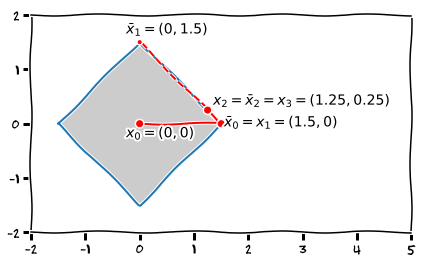
\includegraphics[width=0.75\linewidth]{images/frankwolfesequence.png}
\caption{Frank-Wolfe iteration to solve the program $(P)$ in Example \ref{example:FrankWolfe}.}
\end{figure}
\end{example}
